% ============================================================
% EFML Team 52 — SRUNetHeavy Acceleration
% Compile: lualatex presentation.tex  (twice for cross-refs)
% ============================================================
\documentclass[aspectratio=169,11pt]{beamer}

% ── Theme ───────────────────────────────────────────────────
\usetheme{default}
\usefonttheme{professionalfonts}
\setbeamertemplate{navigation symbols}{}

\definecolor{mainblue}{RGB}{28, 80, 161}
\definecolor{accentblue}{RGB}{14, 116, 144}
\definecolor{accentgreen}{RGB}{5, 130, 80}
\definecolor{hlgreen}{RGB}{220, 248, 232}
\definecolor{hlyellow}{RGB}{255, 251, 220}
\definecolor{lightgray}{RGB}{245, 245, 248}
\definecolor{darkgray}{RGB}{55, 55, 65}

\setbeamercolor{structure}{fg=mainblue}
\setbeamercolor{title}{fg=white, bg=mainblue}
\setbeamercolor{frametitle}{fg=white, bg=mainblue}
\setbeamercolor{block title}{fg=white, bg=mainblue}
\setbeamercolor{block body}{fg=darkgray, bg=lightgray}
\setbeamercolor{block title alerted}{fg=white, bg=accentgreen!90!black}
\setbeamercolor{block body alerted}{fg=darkgray, bg=hlgreen}
\setbeamercolor{block title example}{fg=white, bg=accentblue}
\setbeamercolor{block body example}{fg=darkgray, bg=cyan!8}
\setbeamercolor{normal text}{fg=darkgray}
\setbeamercolor{footline}{fg=white, bg=mainblue!85}

\setbeamertemplate{frametitle}{%
  \nointerlineskip
  \begin{beamercolorbox}[wd=\paperwidth,ht=2.6ex,dp=1.0ex,leftskip=0.6cm,rightskip=0.3cm]{frametitle}%
    \usebeamerfont{frametitle}\insertframetitle%
    \ifx\insertframesubtitle\@empty\else
      \hfill{\small\itshape\insertframesubtitle}%
    \fi
  \end{beamercolorbox}%
}

\setbeamertemplate{footline}{%
  \leavevmode
  \hbox{%
    \begin{beamercolorbox}[wd=.42\paperwidth,ht=2.2ex,dp=0.9ex,leftskip=0.4cm]{footline}%
      {\footnotesize Чубов\,·\,Веселков\,·\,Петухов\enspace|\,EFML~2026}%
    \end{beamercolorbox}%
    \begin{beamercolorbox}[wd=.46\paperwidth,ht=2.2ex,dp=0.9ex,center]{footline}%
      {\footnotesize \insertshorttitle}%
    \end{beamercolorbox}%
    \begin{beamercolorbox}[wd=.12\paperwidth,ht=2.2ex,dp=0.9ex,right,rightskip=0.4cm]{footline}%
      {\footnotesize \insertframenumber\,/\,\inserttotalframenumber}%
    \end{beamercolorbox}%
  }%
}

% ── Packages ────────────────────────────────────────────────
\usepackage{fontspec}
\usepackage{polyglossia}
\setmainlanguage{russian}
\setotherlanguage{english}
\setmainfont{Carlito}
\setsansfont{Carlito}
\setmonofont{DejaVu Sans Mono}[Scale=0.85]
\usepackage{booktabs}
\usepackage{multirow}
\usepackage{array}
\usepackage{graphicx}
\usepackage{xcolor}
\usepackage{colortbl}
\usepackage{tikz}
\usetikzlibrary{positioning}

% ── Metadata ────────────────────────────────────────────────
\title[SRUNetHeavy Acceleration]{Ускорение инференса UNet\\ для задачи Super-Resolution}
\subtitle{Efficient ML — Team 52}
\author[Чубов · Веселков · Петухов]{%
  Артём Чубов \quad Женя Веселков \quad Андрей Петухов%
}
\institute{EFML 2026}
\date{Апрель 2026}

\graphicspath{{results/}}
\newcommand{\hlrow}{\rowcolor{hlgreen}}
\newcommand{\hlyrow}{\rowcolor{hlyellow}}

\begin{document}

% ============================================================
% SLIDE 1 — Title
% ============================================================
\begin{frame}[plain]
  \begin{tikzpicture}[remember picture, overlay]
    \fill[mainblue] (current page.north west) rectangle (current page.south east);
    \fill[accentblue!80] (current page.south west) rectangle +(\paperwidth, 0.5cm);
  \end{tikzpicture}
  \vspace{0.9cm}
  \begin{center}
    {\Large\bfseries\color{white} Ускорение инференса UNet}\\[0.3em]
    {\large\color{white!90} для задачи Super-Resolution~\texttimes 4}\\[0.9em]
    {\normalsize\color{white!75} Efficient ML — Team 52}\\[0.65em]
    \color{white!50}\rule{0.38\textwidth}{0.4pt}\\[0.5em]
    {\small\color{white!80}%
      Артём Чубов \enspace·\enspace Женя Веселков \enspace·\enspace Андрей Петухов}\\[0.25em]
    {\footnotesize\color{white!60} Апрель 2026}
  \end{center}
\end{frame}

% ============================================================
% SLIDE 2 — Pipeline Demo
% ============================================================
\begin{frame}{Задача: Super-Resolution~\texttimes 4}
  \begin{columns}[c]
    \begin{column}{0.58\textwidth}
      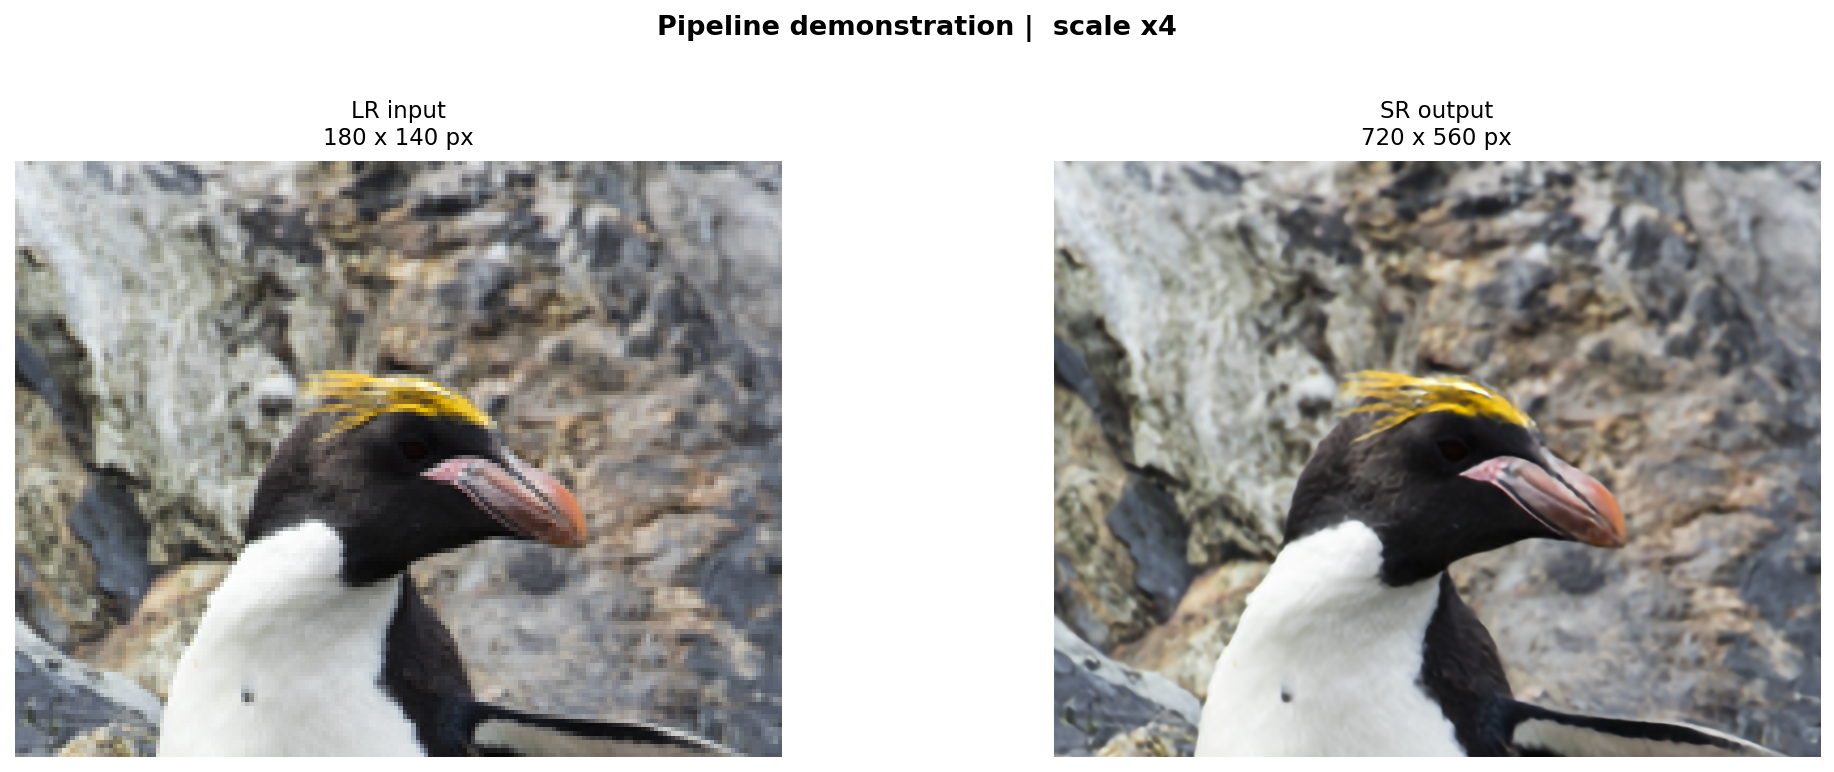
\includegraphics[width=\linewidth]{demo/lr_vs_sr_penguin_head.png}
      \begin{center}
        {\small LR вход (180\texttimes 140~px) \hfill SR выход (720\texttimes 560~px)}
      \end{center}
    \end{column}
    \begin{column}{0.38\textwidth}
      \begin{block}{Что делает модель}
        По Low-Resolution входу восстанавливает детали — масштаб \texttimes 4\\[0.3em]
        LR 256\texttimes 256 → SR 256\texttimes 256\\
        {\footnotesize (вычисления на LR-разрешении)}
      \end{block}
      \vspace{0.4em}
      \begin{block}{Датасет: DIV2K}
        2K HR-фотографии природы\\[0.2em]
        \begin{tabular}{@{}lr@{}}
          Train & 800 изображений \\
          Val   &  50 изображений \\
          Test  &  50 изображений \\
        \end{tabular}\\[0.2em]
        LR on-the-fly: bicubic \,{\small ↓\texttimes 4 → ↑\texttimes 4}
      \end{block}
    \end{column}
  \end{columns}
\end{frame}

% ============================================================
% SLIDE 3 — Model
% ============================================================
\begin{frame}{Модель: SRUNetHeavy}
  \begin{columns}[T]
    \begin{column}{0.48\textwidth}
      \begin{block}{Архитектура}
        \begin{itemize}
          \item U-Net, 5 уровней энкодер/декодер
          \item \textbf{MBResBlock} (inverted residual):\\
                \footnotesize Conv1\texttimes 1 → DWConv3\texttimes 3 → Conv1\texttimes 1
          \item \textbf{SEBlock} в боттлнеке
          \item Глобальный residual
          \item \textbf{GroupNorm} — каналы можно удалять без пересчёта статистик
        \end{itemize}
      \end{block}
    \end{column}
    \begin{column}{0.48\textwidth}
      \begin{alertblock}{Ключевые параметры}
        \renewcommand{\arraystretch}{1.15}
        \footnotesize
        \begin{tabular}{@{}ll@{}}
          Параметры  & \textbf{29.3M} \\
          FLOPs      & 138 GFLOPs \\
          Вход/выход & 256\texttimes 256 → 256\texttimes 256 \\
          Метрика    & SSIM (FP32 ref = \textbf{0.7689}) \\
          Бенчмарк   & CUDA Events, BS=1 \\
        \end{tabular}
      \end{alertblock}
      \vspace{0.4em}
      \begin{exampleblock}{Метрика ускорения}
        Speedup = \textit{baseline latency\,/\,result latency}\\[0.2em]
        Контроль качества: SSIM vs FP32 baseline
      \end{exampleblock}
    \end{column}
  \end{columns}
\end{frame}

% ============================================================
% SLIDE 4 — Summary Results
% ============================================================
\begin{frame}{Главные результаты — все методы}
  \begin{center}
  \footnotesize
  \renewcommand{\arraystretch}{1.08}
  \begin{tabular}{@{}llrrl@{}}
    \toprule
    \textbf{Метод} & \textbf{Precision} & \textbf{Speedup} & \textbf{SSIM} & \textbf{GPU} \\
    \midrule
    Eager baseline      & FP32      & 1.00\texttimes & 0.769 & RTX 3060 \\
    Eager baseline      & FP16      & 1.52\texttimes & 0.769 & RTX 3060 \\
    torch.compile       & FP32      & 1.03\texttimes & 0.769 & RTX 3060 \\
    ORT TensorRT EP     & FP32      & 1.61\texttimes & 0.769 & RTX 3060 \\
    \hlrow
    \textbf{ORT TRT EP}   & \textbf{FP16} & \textbf{3.62\texttimes} & \textbf{0.769} & RTX 3060 \\
    \hlyrow
    \textbf{LSQ PTQ + FP16} & INT8/FP16 & $\approx$1.0\texttimes\,$^*$ & 0.768 & A100 \\
    Struct. pruning 25\% & FP32   & 1.23\texttimes & 0.760 & RTX 8000 \\
    Struct. pruning 50\% & FP32   & 1.57\texttimes & 0.758 & RTX 8000 \\
    \hlrow
    \textbf{Struct. pruning 75\%} & \textbf{FP32} & \textbf{2.27\texttimes} & \textbf{0.760} & RTX 8000 \\
    2:4 sparsity (FP16) & FP16      & 0.84\texttimes & — & A100 \\
    \bottomrule
  \end{tabular}
  \end{center}
  \vspace{0.15em}
  {\footnotesize $^*$ LSQ PTQ: главный выигрыш — сжатие модели в \textbf{4\texttimes} (112~MB~→~28~MB)}
\end{frame}

% ============================================================
% SLIDE 5 — Артём: LSQ PTQ — Method
% ============================================================
\begin{frame}{Артём: Квантизация LSQ — метод}
  \begin{columns}[T]
    \begin{column}{0.52\textwidth}
      \begin{block}{LSQ: Learned Step Size Quantization}
        \textbf{Fake quantization} — форвард симулирует INT8,\\
        веса остаются в float:\\[0.4em]
        \hspace{2em}$\hat{w} = \mathrm{round}(w\,/\,s)\cdot s$\\[0.4em]
        \begin{itemize}
          \item $s$ — learnable per-channel step size
          \item Градиент через \texttt{round}: STE
          \item \textbf{PTQ:} $s$ из статистик весов, finetune не нужен
        \end{itemize}
      \end{block}
      \vspace{0.4em}
      \footnotesize\vspace{0.3em}
      \texttt{LsqConv2d/LsqLinear} — drop-in замена\\[0.1em]
      \texttt{apply\_lsq\_ptq()} — калибровка на val\\[0.1em]
      \texttt{finalize\_lsq()} — экспорт INT8 + FP16 scales
    \end{column}
    \begin{column}{0.44\textwidth}
      \begin{alertblock}{Сжатие модели}
        \renewcommand{\arraystretch}{1.15}
        \begin{tabular}{@{}lrr@{}}
          \toprule
          Формат & Размер & SSIM \\
          \midrule
          FP32     & 111.7~MB & 0.7689 \\
          FP16     &  55.8~MB & 0.7689 \\
          \hlrow
          \textbf{LSQ INT8} & \textbf{28.1~MB} & \textbf{0.7680} \\
          \bottomrule
        \end{tabular}\\[0.3em]
        \textbf{4\texttimes} меньше FP32\\[0.1em]
        SSIM $\Delta = {-}0.0009$ (без finetune)\\[0.2em]
        {\footnotesize INT8 state dict: веса в \texttt{int8} + FP16 scales}
      \end{alertblock}
    \end{column}
  \end{columns}
\end{frame}

% ============================================================
% SLIDE 6 — Артём: LSQ PTQ — Results
% ============================================================
\begin{frame}[shrink=10]{Артём: Квантизация LSQ — результаты}
  \framesubtitle{NVIDIA A100-SXM4-80GB · 256\texttimes 256 · 100 runs}
  \begin{columns}[T]
    \begin{column}{0.54\textwidth}
      \small
      \renewcommand{\arraystretch}{1.22}
      \begin{tabular}{@{}lrrrr@{}}
        \toprule
        \textbf{Config} & \textbf{BS=1} & \textbf{BS=4} & \textbf{BS=16} & \textbf{BS=64} \\
        \midrule
        FP32      & 30.2 ms & 51.0 ms & 128.9 ms & 485.8 ms \\
        FP16      & 26.1 ms & 41.0 ms &  89.3 ms & 306.9 ms \\
        LSQ+FP32  & 41.3 ms & 61.5 ms & 139.5 ms & 496.0 ms \\
        \hlrow
        \textbf{LSQ+FP16} & 37.7 ms & 51.9 ms & 99.9 ms & \textbf{316.8 ms} \\
        \bottomrule
      \end{tabular}
      \vspace{0.4em}
      \footnotesize
      \begin{tikzpicture}[x=0.020cm, y=0.40cm]
        \fill[gray!35]       (0,2) rectangle (111.7,2.65);
        \node[anchor=west,font=\footnotesize] at (2,2.325) {FP32 \ 111.7 MB};
        \fill[mainblue!55]   (0,1) rectangle ( 55.8,1.65);
        \node[anchor=west,font=\footnotesize] at (2,1.325) {FP16 \ 55.8 MB};
        \fill[accentgreen!70](0,0) rectangle ( 28.1,0.65);
        \node[anchor=west,font=\footnotesize] at (2,0.325) {\textbf{INT8 28.1 MB}};
      \end{tikzpicture}
    \end{column}
    \begin{column}{0.42\textwidth}
      \begin{block}{Выводы}
        \begin{itemize}
          \item LSQ+FP16 при BS=64 → \textbf{0.97\texttimes} vs FP16
          \item Fake quant не ускоряет:\\
                вычисления в float
          \item Выигрыш: \textbf{хранение} (4\texttimes)
          \item Для speedup нужны INT8-ядра\\
                \footnotesize{(TRT INT8, torch.ao)}
        \end{itemize}
      \end{block}
    \end{column}
  \end{columns}
\end{frame}

% ============================================================
% SLIDE 7 — Женя: Baseline & torch.compile
% ============================================================
\begin{frame}{Женя: Baseline и компиляция}
  \framesubtitle{SRUNetHeavy 29M · RTX 3060 · BS=1 · 50 runs}
  \begin{columns}[T]
    \begin{column}{0.50\textwidth}
      \small
      \renewcommand{\arraystretch}{1.2}
      \begin{tabular}{@{}llrr@{}}
        \toprule
        \textbf{Метод} & \textbf{Prec.} & \textbf{Latency} & \textbf{Speedup} \\
        \midrule
        Eager PyTorch       & FP32 & 48.1 ms & 1.00\texttimes \\
        Eager PyTorch       & FP16 & 31.7 ms & 1.52\texttimes \\
        \midrule
        torch.compile       & FP32 & 46.6 ms & 1.03\texttimes \\
        ORT CUDA EP         & FP32 & 46.1 ms & 1.04\texttimes \\
        \hlrow
        ORT TRT EP          & FP32 & 29.8 ms & 1.61\texttimes \\
        \hlrow
        \textbf{ORT TRT EP} & \textbf{FP16} & \textbf{13.3 ms} & \textbf{3.62\texttimes} \\
        \bottomrule
      \end{tabular}
      \vspace{0.3em}\\
      {\footnotesize Throughput TRT FP16: \textbf{75.2 img/s} vs 20.8 img/s (Eager FP32)}
    \end{column}
    \begin{column}{0.46\textwidth}
      \begin{block}{torch.compile — почему мало?}
        \small
        Triton не находит fusion для\\
        \texttt{GroupNorm + GELU + DWConv3\texttimes 3}\\[0.25em]
        TensorRT кодирует их custom plugins\\
        → kernel launch overhead ↓↓
      \end{block}
      \vspace{0.2em}
      \begin{alertblock}{TRT FP16 — откуда 3.62\texttimes?}
        \small
        \begin{itemize}
          \item 1\texttimes 1 Conv = GEMM → Tensor Cores
          \item Fusion GroupNorm+GELU+Conv
          \item Вдвое меньше DRAM-трафика
        \end{itemize}
      \end{alertblock}
    \end{column}
  \end{columns}
\end{frame}

% ============================================================
% SLIDE 8 — Женя: TensorRT vs UNetSR
% ============================================================
\begin{frame}{Женя: TensorRT — сравнение моделей}
  \begin{columns}[T]
    \begin{column}{0.50\textwidth}
      \footnotesize\renewcommand{\arraystretch}{1.15}
      \begin{tabular}{@{}llrr@{}}
        \toprule
        \textbf{Модель} & \textbf{Метод} & \textbf{Latency} & \textbf{Speedup} \\
        \midrule
        \multirow{3}{*}{SRUNetHeavy}
          & Eager FP32    & 48.1 ms  & 1.00\texttimes \\
          & TRT FP32      & 29.8 ms  & 1.61\texttimes \\
          & \textbf{TRT FP16} & \textbf{13.3 ms} & \textbf{3.62\texttimes} \\
        \midrule
        \multirow{3}{*}{UNetSR}
          & Eager FP32    & 119.7 ms & 1.00\texttimes \\
          & TRT FP32      &  90.6 ms & 1.32\texttimes \\
          & \textbf{TRT FP16} & \textbf{30.8 ms} & \textbf{3.87\texttimes} \\
        \bottomrule
      \end{tabular}
    \end{column}
    \begin{column}{0.46\textwidth}
      \begin{alertblock}{Почему SRUNetHeavy лучше реагирует на TRT FP32?}
        \small
        ×1.61 vs ×1.32 у UNetSR\\[0.2em]
        MBResBlock: больше 1×1 conv относительно DWConv → fusion GroupNorm+GELU+Conv1×1 важнее
      \end{alertblock}
      \vspace{0.3em}
      \begin{exampleblock}{Ограничение DWConv}
        \small
        DWConv3×3 \textbf{не использует Tensor Cores}\\
        (TC нужны матрицы ≥16×16)\\[0.15em]
        FP16 ускоряется за счёт bandwidth, а не вычислений
      \end{exampleblock}
    \end{column}
  \end{columns}
\end{frame}

% ============================================================
% SLIDE 9 — Женя: Roofline Analysis
% ============================================================
\begin{frame}{Женя: Roofline-анализ}
  \framesubtitle{SRUNetHeavy · RTX 3060}
  \begin{columns}[c]
    \begin{column}{0.56\textwidth}
      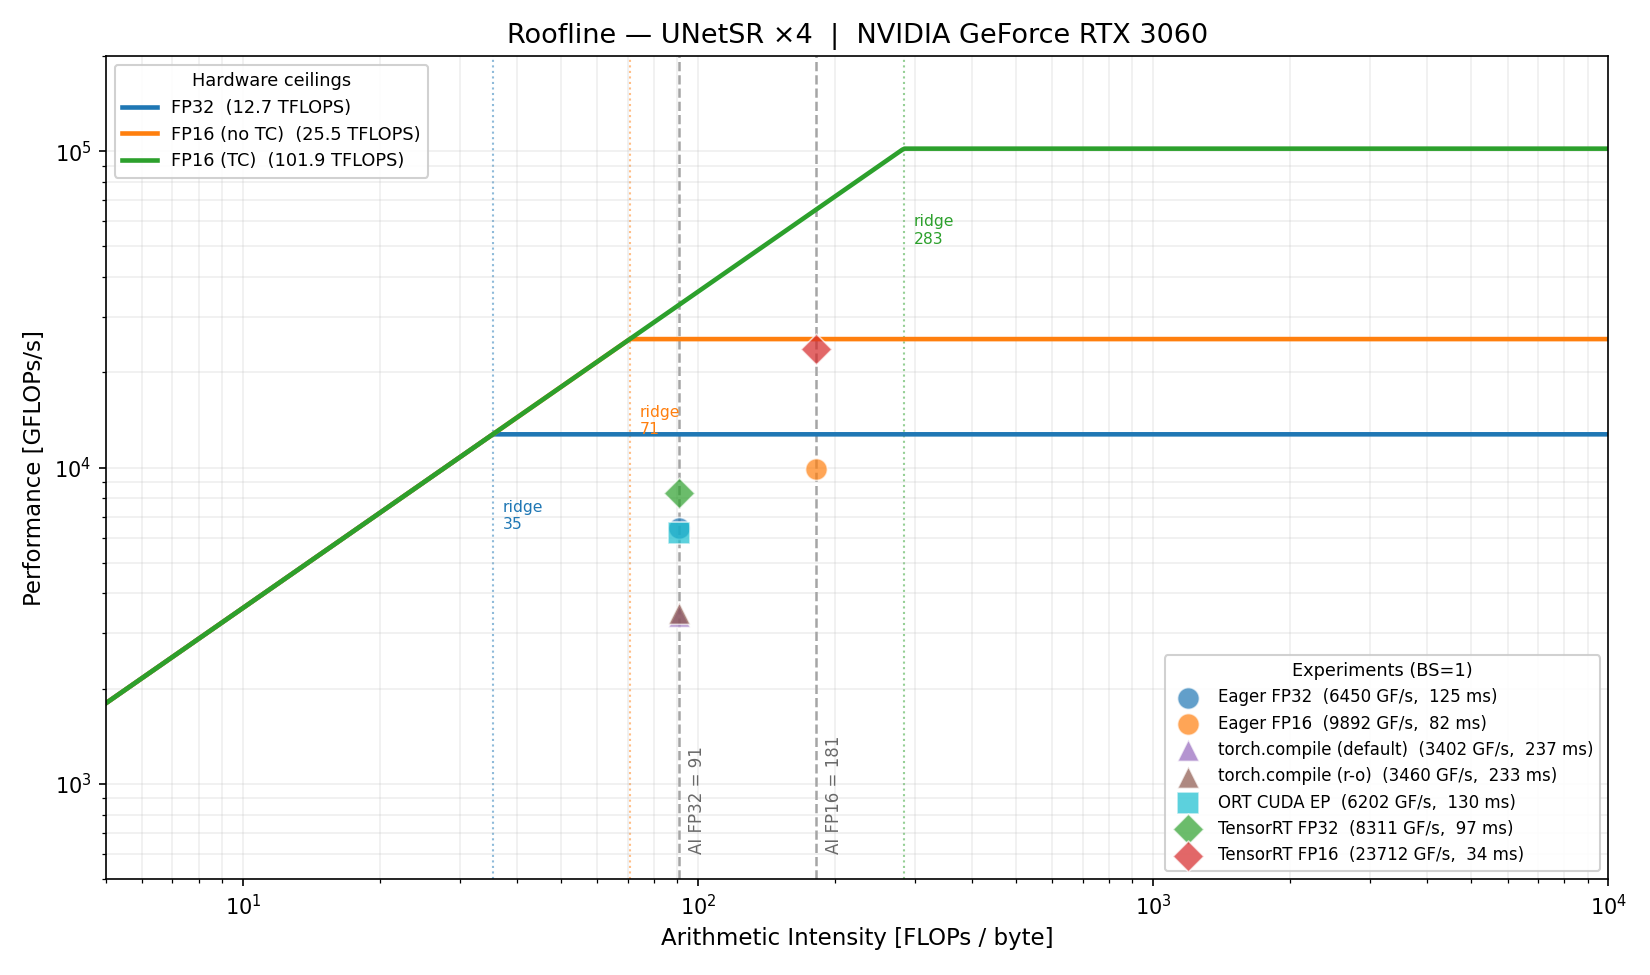
\includegraphics[width=\linewidth]{zhenya-results/roofline_rtx3060.png}
    \end{column}
    \begin{column}{0.40\textwidth}
      \small
      \begin{block}{Arithmetic Intensity}
        \renewcommand{\arraystretch}{1.1}
        \begin{tabular}{@{}lrl@{}}
          \toprule
           & AI & режим \\
          \midrule
          FP32 ridge  & 35   & — \\
          FP16 TC ridge & 283 & — \\
          \midrule
          AI FP32  & 210 & compute-bound \\
          AI FP16  & 420 & compute-bound \\
          \bottomrule
        \end{tabular}
      \end{block}
      \vspace{0.35em}
      \textbf{Почему лишь 22\% от пика?}\\[0.1em]
      DWConv3\texttimes 3 — каналы независимо, warp occupancy низкий
      \vspace{0.2em}
      \begin{alertblock}{}
        \footnotesize
        Eager FP32: 22\% пика\\
        TRT FP32:\phantom{x} 36\% пика\\
        TRT FP16:\phantom{x} 10\% TC-пика
      \end{alertblock}
    \end{column}
  \end{columns}
\end{frame}

% ============================================================
% SLIDE 10 — Андрей: Structural Pruning — Idea
% ============================================================
\begin{frame}[shrink=10]{Андрей: Структурное прунирование — идея}
  \begin{columns}[T]
    \begin{column}{0.50\textwidth}
      \begin{block}{Expand-Channel Pruning}
        В каждом MBResBlock физически удаляем каналы expand 1\texttimes 1 conv с наименьшей L1-нормой\\[0.2em]
        \textbf{U-Net топология не нарушается:} только \texttt{mid\_ch} уменьшается
      \end{block}
      \vspace{0.2em}
      \begin{exampleblock}{Почему даёт реальный speedup}
        \begin{itemize}
          \item Тензоры меньше физически — не нужны sparse kernels
          \item GroupNorm — каналы удаляются без пересчёта
          \item Finetune (10 эпох) восстанавливает SSIM
        \end{itemize}
      \end{exampleblock}
    \end{column}
    \begin{column}{0.46\textwidth}
      \begin{alertblock}{Результаты: 75\% + finetune}
        \footnotesize\renewcommand{\arraystretch}{1.1}
        \begin{tabular}{@{}lrr@{}}
          \toprule
          & До & После \\
          \midrule
          Параметры & 29.3M & \textbf{8.4M} \\
          Latency BS=1 & 34.2 ms & \textbf{15.1 ms} \\
          Speedup BS=1 & — & \textbf{2.27\texttimes} \\
          SSIM & 0.7689 & 0.7598 \\
          \bottomrule
        \end{tabular}\\[0.15em]
        Модель в \textbf{3.5\texttimes} меньше · SSIM \textbf{−0.009}
      \end{alertblock}
    \end{column}
  \end{columns}
\end{frame}

% ============================================================
% SLIDE 11 — Андрей: Structural Pruning — Plots
% ============================================================
\begin{frame}{Андрей: Структурное прунирование — результаты}
  \begin{center}
    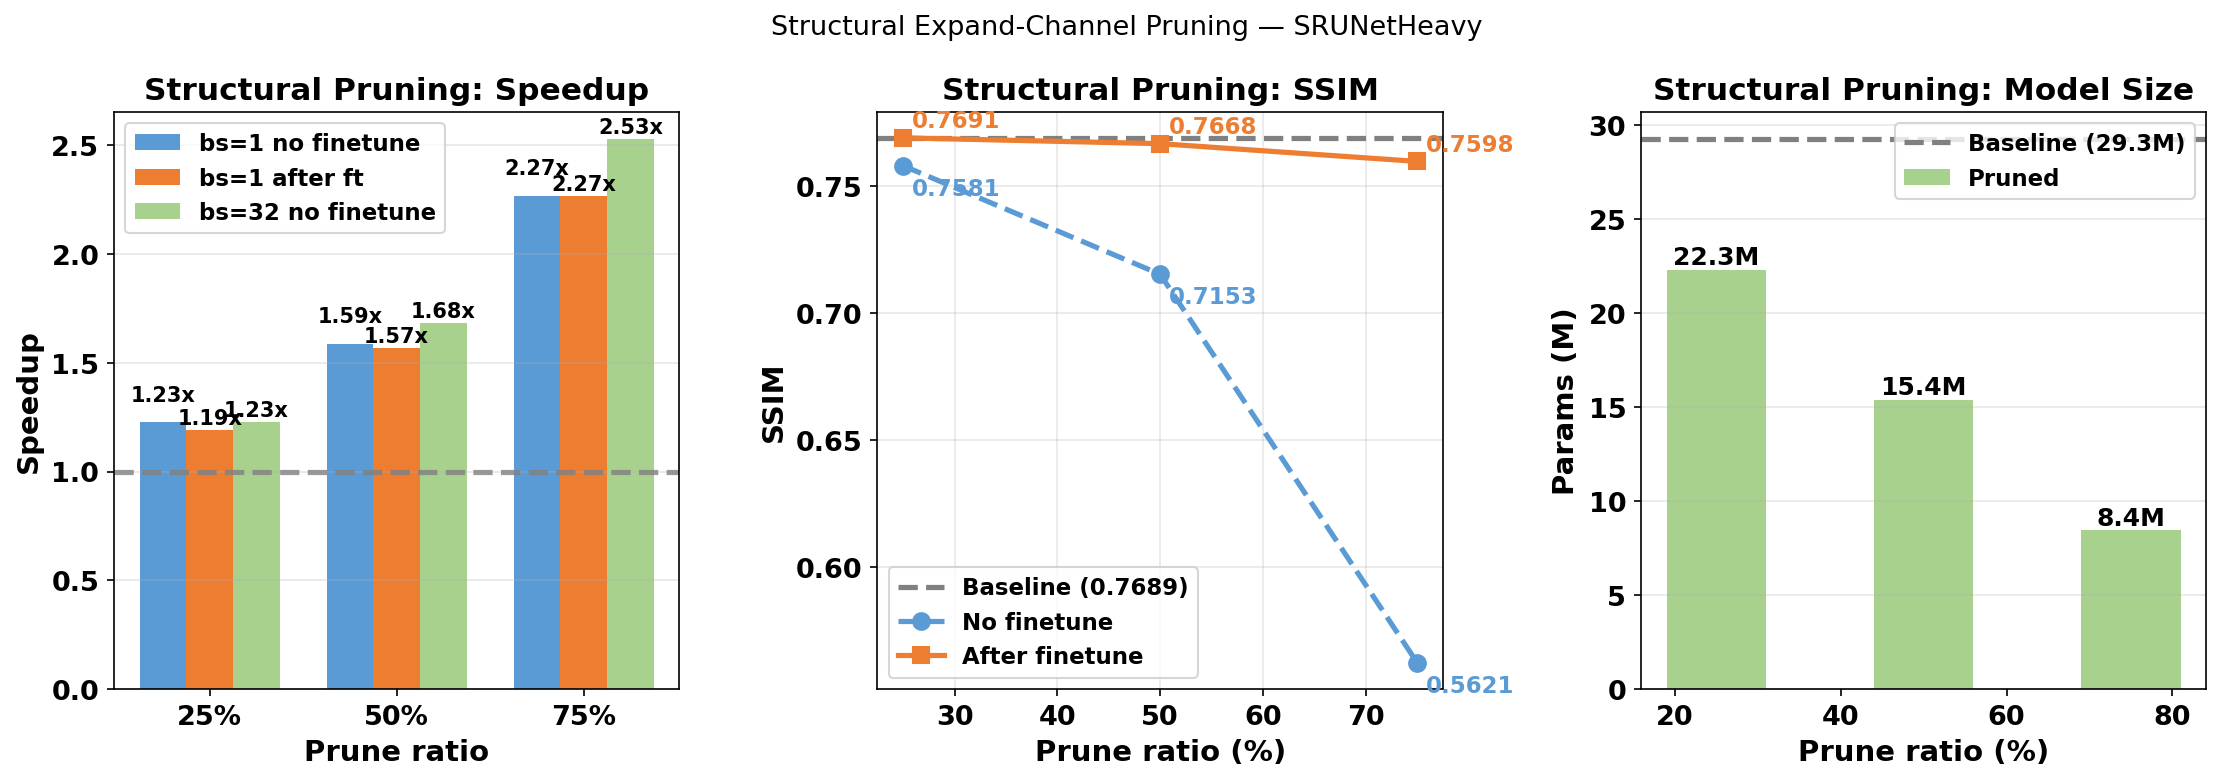
\includegraphics[width=0.90\linewidth]{plots/andrey/structural_pruning.png}
  \end{center}
  \vspace{0.15em}
  \begin{center}
    \footnotesize\renewcommand{\arraystretch}{1.1}
    \begin{tabular}{@{}lrrrr@{}}
      \toprule
      \textbf{Прунирование} & \textbf{Speedup BS=1} & \textbf{Speedup BS=32} & \textbf{SSIM (ft)} & \textbf{Params} \\
      \midrule
      25\% + finetune & 1.23\texttimes & 1.23\texttimes & 0.760 & 22.3M \\
      50\% + finetune & 1.57\texttimes & 1.68\texttimes & 0.758 & 15.4M \\
      \hlrow
      \textbf{75\% + finetune} & \textbf{2.27\texttimes} & \textbf{2.53\texttimes} & \textbf{0.760} & \textbf{8.4M} \\
      \bottomrule
    \end{tabular}
  \end{center}
\end{frame}

% ============================================================
% SLIDE 12 — Андрей: Magnitude Pruning
% ============================================================
\begin{frame}{Андрей: Magnitude Pruning}
  \begin{columns}[c]
    \begin{column}{0.62\textwidth}
      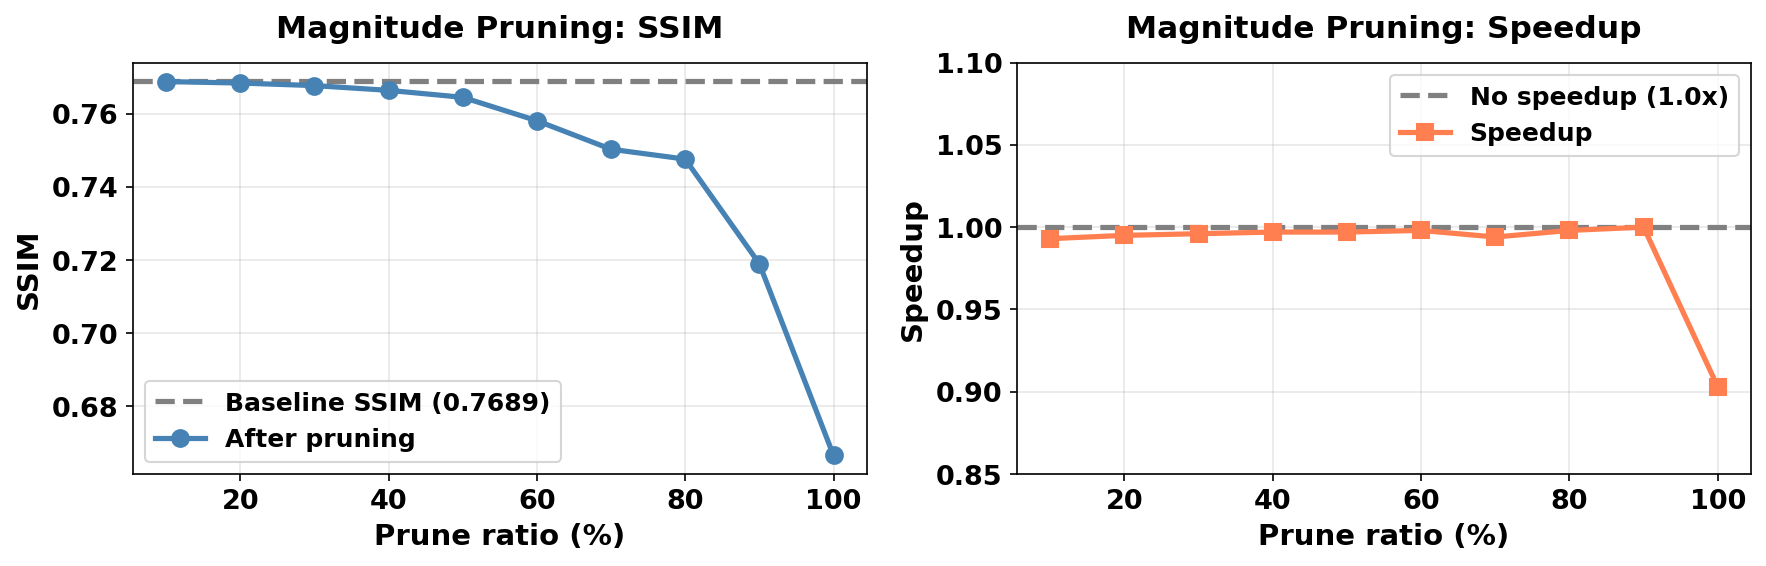
\includegraphics[width=\linewidth]{plots/andrey/magnitude_pruning.png}
    \end{column}
    \begin{column}{0.34\textwidth}
      \begin{block}{Метод}
        \small
        Обнуляем N\% наименьших весов 1\texttimes 1 Conv2d через \texttt{global\_unstructured}
      \end{block}
      \vspace{0.3em}
      \begin{alertblock}{Speedup ≈ 1.0\texttimes}
        \small
        Тензоры остаются \textbf{dense} — GPU исполняет те же CUDA-ядра с теми же матрицами\\[0.15em]
        Нули перемножаются, а не пропускаются
      \end{alertblock}
    \end{column}
  \end{columns}
\end{frame}

% ============================================================
% SLIDE 13 — Андрей: 2:4 Semi-structured Sparsity
% ============================================================
\begin{frame}[shrink=10]{Андрей: 2:4 Semi-structured Sparsity}
  \begin{columns}[c]
    \begin{column}{0.60\textwidth}
      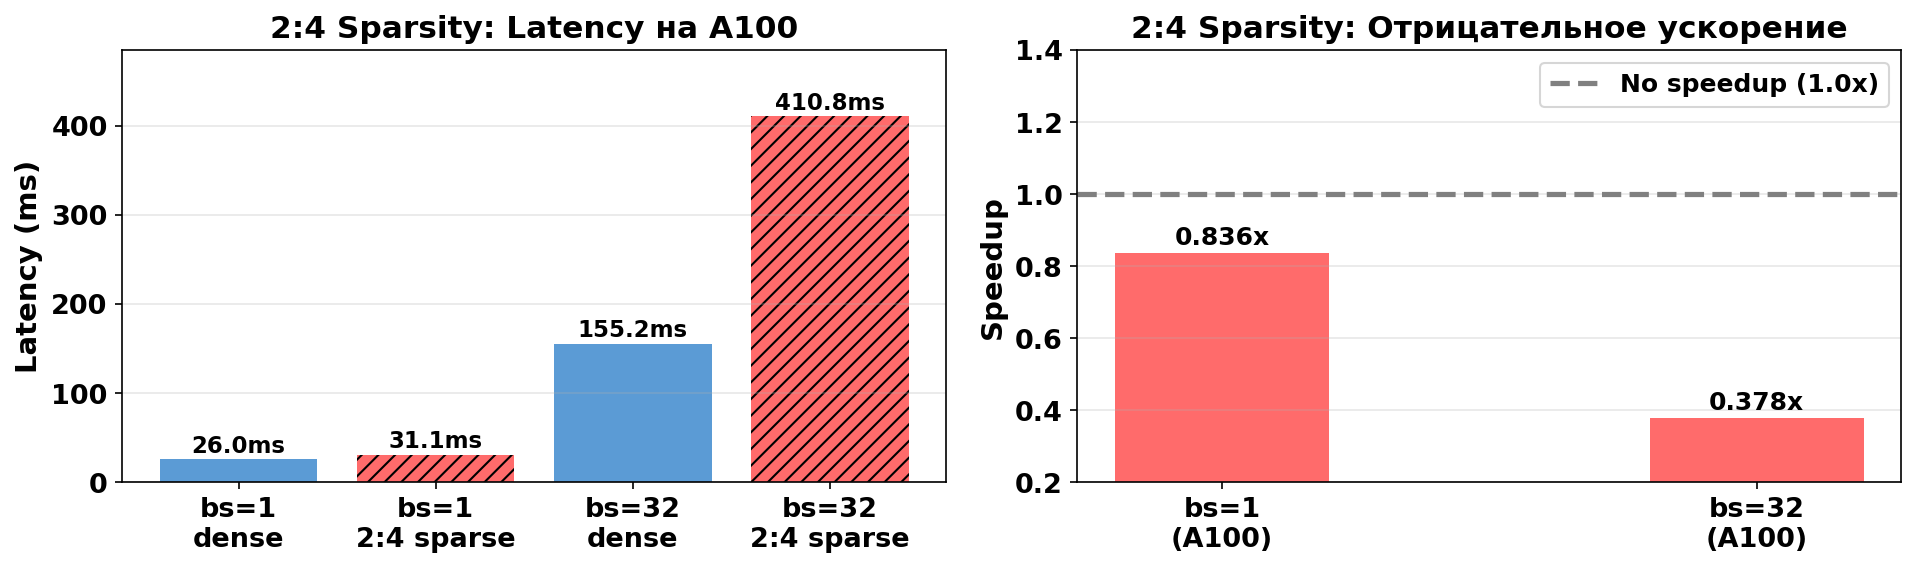
\includegraphics[width=\linewidth]{plots/andrey/sparse_244.png}
    \end{column}
    \begin{column}{0.36\textwidth}
      \begin{block}{Метод}
        \small
        В каждой группе из 4 весов ровно 2 обнуляются (по наименьшей норме).\\[0.2em]
        \texttt{to\_sparse\_semi\_structured} + cuSPARSELt
      \end{block}
      \vspace{0.35em}
      \begin{alertblock}{Почему нет speedup}
        \small
        \begin{itemize}
          \item cuSPARSELt — только \textbf{Ampere (sm\_80+)}, RTX~8000 = Turing
          \item На A100: матрицы 1\texttimes 1 Conv слишком малы — overhead перевешивает
          \item BS=1: \textbf{0.84\texttimes}, BS=32: \textbf{0.38\texttimes}
        \end{itemize}
      \end{alertblock}
    \end{column}
  \end{columns}
\end{frame}

% ============================================================
% SLIDE 14 — Андрей: Group Conv
% ============================================================
\begin{frame}{Андрей: Grouped Convolutions}
  \begin{columns}[c]
    \begin{column}{0.58\textwidth}
      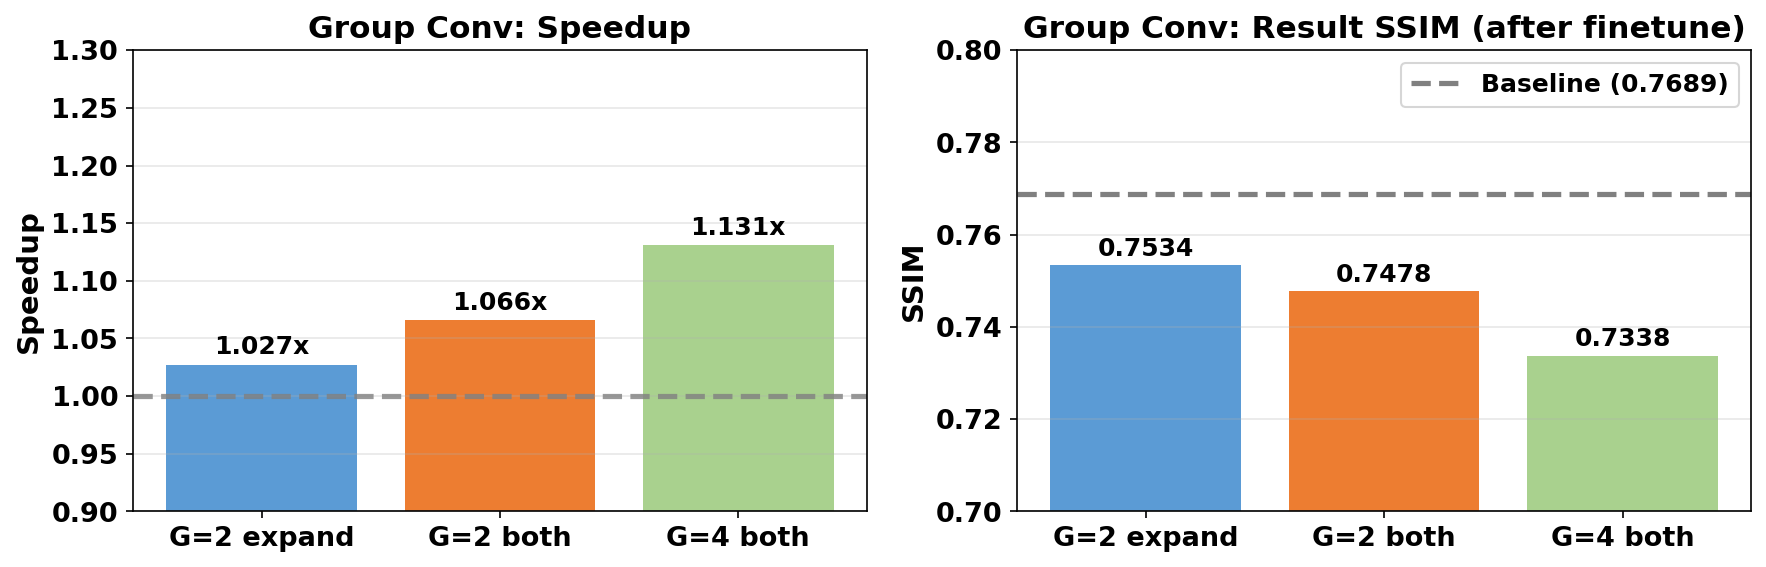
\includegraphics[width=\linewidth]{plots/andrey/group_conv.png}
    \end{column}
    \begin{column}{0.38\textwidth}
      \begin{block}{Метод}
        \small
        expand/project 1\texttimes 1 Conv → grouped conv (G=2 или G=4).\\[0.2em]
        FLOPs \(\div\) G, но CUDA matmul overhead ограничивает реальный speedup.
      \end{block}
      \vspace{0.4em}
      \begin{exampleblock}{Сравнение}
        \small
        G=4 both: \textbf{1.13\texttimes}, SSIM \({-}0.035\)\\[0.15em]
        Struct. 75\%: \textbf{2.27\texttimes}, SSIM \({-}0.009\)\\[0.3em]
        → Структурное прунирование превосходит по обеим метрикам
      \end{exampleblock}
    \end{column}
  \end{columns}
\end{frame}

% ============================================================
% SLIDE 15 — Conclusions
% ============================================================
\begin{frame}{Выводы}
  \begin{columns}[T]
    \begin{column}{0.48\textwidth}
      \begin{alertblock}{Лучшие результаты}
        \footnotesize\renewcommand{\arraystretch}{1.1}
        \begin{tabular}{@{}lll@{}}
          \toprule
          \textbf{Цель} & \textbf{Метод} & \textbf{Итог} \\
          \midrule
          Макс. ускорение    & TRT FP16      & \textbf{3.62\texttimes} \\
          Без потерь SSIM    & TRT FP16      & SSIM = 0.769 \\
          Сжатие модели      & LSQ PTQ       & \textbf{4\texttimes} \\
          Speed+компактность & Struct. 75\%  & \textbf{2.27\texttimes} \\
          \bottomrule
        \end{tabular}
      \end{alertblock}
      \vspace{0.2em}
      \begin{center}
        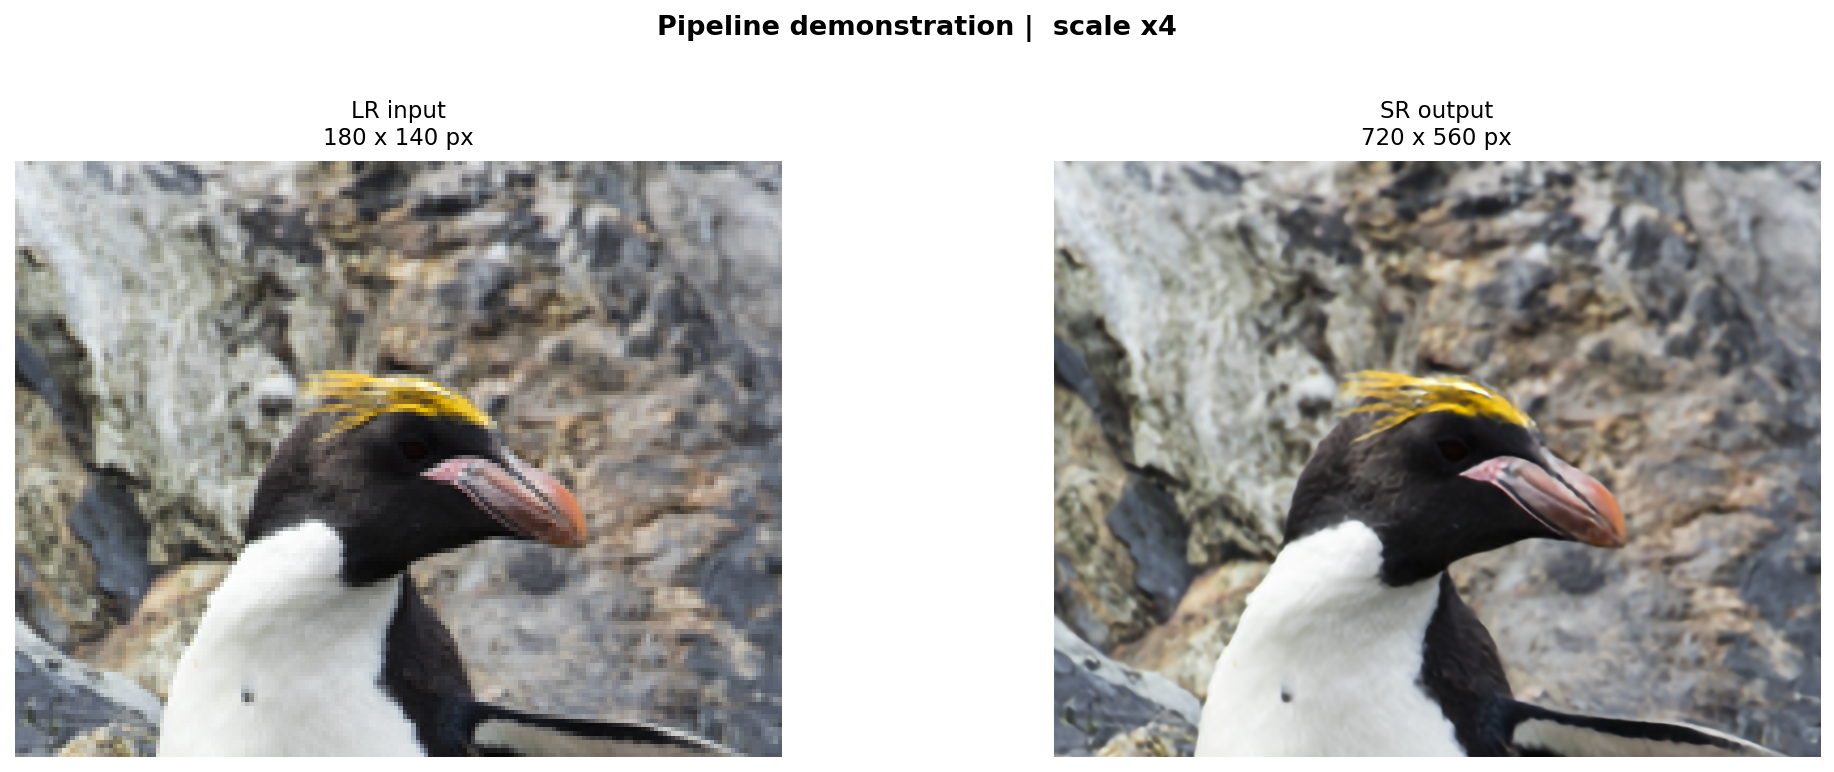
\includegraphics[height=2.2cm]{demo/lr_vs_sr_penguin_head.png}
      \end{center}
    \end{column}
    \begin{column}{0.48\textwidth}
      \begin{block}{Ключевые наблюдения}
        \small
        \begin{itemize}
          \item \textbf{torch.compile} — минимальный выигрыш:\\Triton не фьюзит GroupNorm+GELU+DWConv
          \item \textbf{TensorRT} — лучший бэкенд: fusion + Tensor Cores
          \item \textbf{LSQ PTQ} — 4\texttimes меньше, но без INT8-ядер не ускоряет
          \item \textbf{Struct. pruning} — лучший трейдофф, любой GPU
          \item \textbf{2:4 sparsity} — нужен Ampere+, малые матрицы убыточны
        \end{itemize}
      \end{block}
    \end{column}
  \end{columns}
\end{frame}

\end{document}
